\chapter{Parameter Estimation}\label{Chapter:ParameterEstimation}

Assume we have a parametric model $(\Omega, \mathcal A, \Pr)$ for real independent random  variables $X$ and $\bm X = (X_1,X_2,\dots)$.
The distribution of $X$ is indexed by $\bm \theta\in\bm \Theta\subset \mathbbm R^p$, where $p\geq 1$ is the dimension of the parametric space $\bm \Theta$.

What can we say about $\bm \theta$ using the sample $\bm X$?
This is parametric statistical inference!

We will later need an additional ingredient: expected values of transformations of the random variable $X$:
\begin{equation}
\operatorname{E}\bm\psi(X) = \big(
\operatorname{E}\psi_1(X), \operatorname{E}\psi_2(X), \dots, \operatorname{E}\psi_p(X)
\big),
\label{eq:ExpectedValues}
\end{equation}
where each $\psi_j$ is a measurable function $\psi_j\colon \mathbbm R\to\mathbbm R$.
Each element of~\eqref{eq:ExpectedValues} is given by
\begin{equation}
\operatorname{E}\psi_j(X) = 
	\int_{\mathbbm R} \psi_j(x) dF(x),
\end{equation}
and $F$ is the cumulative distribution function of $X$.
If $\psi(X)=X^k$, we say that $\operatorname{E}X^k$ is the $k$-th order moment of $X$ (if it exists).

The quantity $\operatorname{E}(X-\operatorname{E}X)^k$ is called ``the central moment'' of $X$, if it exists.
The second central moment $\operatorname{E}(X-\operatorname{E}X)^2 = \operatorname{E}X^2-(\operatorname{E}X)^2$ is called ``the variance'' of $X$.
We denote it $\operatorname{Var}X$

In general, $\operatorname{E}X^k\neq (\operatorname{E}X)^k$.

\section{Models}

We will use a few models as examples.
The interested reader is referred to, among other references, to the books by \citet{johnson_discrete} for discrete distributions, and by \citet{johnson_continuous2} for continuous random variables.

\subsection{The Bernoulli distribution}\label{Sec:Bernoulli}

This is the basic discrete distribution.
It models the outcome of a dichotomic random experiment, i.e., with only two possible outcomes: failure ($0$) or success ($1$).
Denote $N\sim\text{Be}(p)$ a random variable with Bernoulli distribution and probability $0\leq p\leq 1$.
The vector of probabilities is $(1-p,p)$.

\subsection{The Negative Binomial distribution}\label{Sec:NegativeBinomial}

This discrete distribution is basilar in the construction of the $\mathcal K$ law.
We say that $N\sim\text{NB}(r,p)$ has negative binomial distribution if its vector of probabilities is given by
$$
\Pr(N=n) = {{k+r-1}\choose{k}} p^k (1-p)^r,
$$
com $0<p<1$ and $1\leq n\leq k$.

This is the distribution that models the probability of having to wait until the $n$th Bernoulli trial with probability $p$ of success until we observe exactly $r$ failures.

\subsection{The Uniform distribution}
We say that $X\sim\mathcal U_{(0,\theta)}$, $\theta>0$ has uniform distribution on the interval $(0,\theta)$ when its density is
\begin{equation}
f_U(u;\theta) = \frac{1}{\theta} \mathbbm 1_{(0,\theta)} (u).
\label{eq:DensUniform}
\end{equation}
With this, we have that the $k$-order moment of $X$ is
\begin{equation}
\operatorname{E}U^k = \int_{\mathbbm R}\frac{1}{\theta} \mathbbm 1_{(0,\theta)} u^k d(u) du = 
\int_{0}^{\theta} \frac1\theta u^k du = 
\frac{1}{k+1} \theta^k.
\label{eq:MomentsUniform}
\end{equation}

Its cumulative distribution function is
\begin{equation}
F_U(u;\theta) = 
	\begin{cases}
	0 				& \text{if } u\leq 0,\\
	\theta^{-1} 	& \text{if } 0< u < \theta,\\
	1 				& \text{otherwise.}
	\end{cases}
\label{eq:CDFUniform}
\end{equation}

\subsection{The Gaussian distribution}

We say that $X\sim N(\mu,\sigma^2)$ follows a Gaussian distribution with mean $\mu\in\mathbbm R$ and variance $\sigma^2$ if the density that characterizes its distribution is
\begin{equation}
f_G(x;\mu,\sigma^2) = \frac{1}{\sqrt{2\pi}\sigma} \exp\Big\{
-\frac{1}{2\sigma^2} \big(x - \mu)^2
\Big\}.
\end{equation}
Its first and second moment are $\operatorname{E}X=\mu$ and
$\operatorname{E}X^2=\mu^2+\sigma^2$.

We don't know explicit expressions for its cumulative distribution function, but it is widely implemented in almost every statistical platform.

\subsection{Mixture of Gaussian distributions}

A mixture of $p$ Gaussian models is characterized by the density
\begin{equation}
f_{\text{MG}}(x;\bm p,\bm \mu, \bm \sigma^2) = 
\sum_{j=1}^{p}
\frac{p_j}{\sqrt{2\pi}\sigma_j} \exp\Big\{
-\frac{1}{2\sigma_j^2} \big(x - \mu_j)^2 \Big\},
\label{eq:DensMixtureGaussian}
\end{equation}
where $\bm p=(p_1,p_2, \dots, p_p)$ is the vector of probabilities,
$\bm \mu = (\mu_1, \mu_2,\dots, \mu_p)$ is the vector of means,
and
$\bm \sigma^2 = (\sigma^2_1, \sigma^2_2,\dots, \sigma^2_ p)$ is the vector of variances.
In this way, the parameter space is $\bm \Theta =
\mathcal S^p\times \mathbbm R^p \times \mathbbm R_+^p$, where
$\mathcal S^p$ is the surface of the $p$-dimensional simplex.
This space is a subset of $\mathbbm R^{(p-1)p^2}$. 
We denote this situation $X\sim \text{MG}(\bm p, \bm \mu, \bm \sigma^2)$.

Using the fact that the random components are independent, it is immediate that
$\operatorname{E}X = \sum_{j=1}^{p} p_j\mu_j$ and that
$\operatorname{Var}X = \sum_{j=1}^{p} p_j^2\sigma^2_j$.

\subsection{The (SAR) Gamma distribution}

The Gamma distribution, in the usual parametrization for SAR data $Z\sim\Gamma(L,\mu)$, with $L,\mu>0$ is characterized by the density
\begin{equation}
f_\Gamma(z;L,\mu) = \frac{L^L}{\mu^{L}\Gamma(L)} z^{L-1} 
	\exp\big\{ -L z / \mu
	\big\}.
\label{eq:SARGammaDensity}
\end{equation}
With this, the first- and second-order moments of $Z$ are
$\operatorname{E}Z=\mu$,
and 
$\operatorname{Var}Z=\mu^2/L$,
respectively.

As for the Gaussian distribution, in general, we do not have explicit expressions for its cumulative distribution function, being the exponential case ($L=1$) an exception.

This is a good model for intensity SAR observations over areas with no texture.
The multiplicative model says the observed return $Z$ is the product of two independent random variables:
$X$, the backscatter, and
$Y$, the speckle.
The speckle can be modeled by a Gamma random variable with shape parameter $L\geq1$ (the number of looks) and unitary mean.

If the area under observation has constant backscatter ($X=\mu$), then the return $Z\sim\Gamma(\mu,L)$.

\subsection{The Reciprocal Gamma distribution}

When the backscatter varies in the observed area we say that the area has texture.
A very flexible model for the backscatter is the Reciprocal Gamma law\cite{frery96}, which is characterized by the density
\begin{equation}
f_Y(y;\alpha,\gamma)= \frac{1}{\gamma^\alpha \Gamma(\alpha)}
y^\alpha \exp\big\{-\gamma/y\big\},
\label{eq:IGDensity}
\end{equation}
where $\alpha<0$ is the texture, and
$\gamma>0$ is the scale.
We denote this situation $Y\sim \Gamma^{-1}(\alpha,\gamma)$.

\subsection{The GI0 distribution}

Assuming that the backscatter is $X\sim\Gamma^{-1}(\alpha,\gamma)$,
the speckle is $Y\sim\Gamma(1,L)$, and that they are independent random variables, we have that the return follows a GI0 distribution\cite{GeodesicDistanceGI0JSTARS,ParameterEstimationSARStochasticDistancesKernels}, denoted $Z\sim\mathcal G_I^0(\alpha,\gamma,L)$, whose density is
\begin{equation}
f_Z(z;\alpha,\gamma,L) = \frac{L^L \Gamma(L-\alpha)}{\gamma^\alpha \Gamma(L) \Gamma(\alpha)}
\frac{z^L}{(\gamma+Lz)^\alpha}.
\end{equation}

The $k$-order moment of $Z$ is given by
\begin{equation}
\operatorname{E}Z^k = \Big(\frac{\gamma}{L}\Big)^k
\frac{\Gamma(-\alpha-k)}{\Gamma(-\alpha)}
\frac{\Gamma(L+k)}{\Gamma(L)},
\end{equation}
provided $k>-\alpha$ and infinite otherwise.

\section{Inference by analogy}

Inference by analogy\cite{manski_analog} is inspired by the Law of Large Numbers, that states that (under relatively mild conditions) holds that
\begin{equation}
\lim_{n\to\infty}\frac1n\sum_{i=1}^{n} \psi(X_i) = 
\operatorname{E}\psi(X),
\label{eq:LLN}
\end{equation}
provided $X,X_1,X_2,\dots$ are independent identically distributed random variables.

With this in mind, and assuming one has a large sample, it seems reasonable to equate sample quantities (the left hand side) and parametric expressions (the right hand side).

When we have $p$ parameters, i.e. $\bm \theta\in\Theta\subset\mathbbm R^p$, we need $p$ linearly independent equations to form an estimator of $\bm \theta$.

\subsection{The Uniform distribution}

Using~\eqref{eq:MomentsUniform} with we can set, for instance, $k=1$ and obtain $\operatorname{E}U=\theta/2$.
With this, our first-order moment estimator for $\theta$ is $\widehat{\theta}_1=2n^{-1}\sum_{i=1}^n U_i$.
But we can also set $k=2$ and obtain a second-order moment estimator, using $\operatorname{E}U^2=\theta^3$ it is immediate that
$\widehat{\theta}_2=\sqrt{3n^{-1}\sum_{i=1}^{n} U_i^2}$.
In fact, the $k$-order moment estimator of $\theta$ based on a sample of size $n$ is
\begin{equation}
\widehat{\theta}_k = \sqrt[k]{\frac{k+1}{n} \sum_{i=1}^{n} U_i^k}.
\end{equation}

This multiplicity of possible analogy estimators gives great flexibility to the method, but it is also one of its weaknesses: the lack of unicity.
Another drawback is that little is known about estimators obtained by this procedure, apart that they are consistent, i.e., that~\eqref{eq:LLN} grants that they converge in probability to the true parameter value.

A more serious problem is that an estimator obtained by this procedure may lead to a model for which observations are unfeasible (and, remember, observations are \emph{correct}).
See, for example, the sample $\bm x=(0.05, 0.15, 1)$.
Its sample mean is $1.2/3=0.4$, therefore the estimate is $\widehat{\theta}_1=0.8$, but the third observation is unfeasible under the $\mathcal U_{(0,0.8)}$ distribution!

By the way, notice an important difference.
We refer to an \emph{estimator} when it is a random variable $\widehat{\theta}(X_1, X_2, \dots)$, and to an \emph{estimate} when the data have been observed $\widehat{\theta}(x_1, x_2, \dots)$ and, thus, is a fixed quantity.

\subsection{The Gaussian distribution}

Using $\operatorname{E}X=\mu$ we obtain $\widehat{\mu}=n^{-1}\sum_{i=1}^{n} X_i$.
Since $\operatorname{E}X^2=\mu^2+\sigma^2$, we have that $\sigma^2=\operatorname{E}X^2-\mu^2$.
We already have an estimator for $\mu$, and also for $\mu^2$, then one estimator for $\sigma^2$ is $\widehat{\sigma}^2=n^{-1}\sum_{i=1}^{n}X_i^2-\widehat{\mu}^2 = n^{-1}\sum_{i=1}^{n}(X_i-\widehat{\mu})^2$.

Other estimators could be formed with higher-order moments $k=3,4\dots$, but we will always need two linearly independent equations to estimate $\bm\theta=(\mu,\sigma^2)$.

\subsection{Mixture of Gaussian distributions}

We need $(p-1)p^2$ linearly independent equations to estimate $\bm{\theta} = (\bm p, \bm \mu, \bm \sigma^2)$.
This approach is not very effective, because results in serious numerical problems.

\subsection{The (SAR) Gamma distribution}

Using $\E(Z)=\mu$ we propose $\widehat{\mu}=n^{-1}\sum_{i=1}^n Z_i$,
and with 
$\operatorname{Var}(Z)=\mu^2/L$, we can estimate $\widehat L=\widehat{\mu}^2 / (n^{-1}\sum_{i=1}^n (Z_i - \widehat{\mu})^2)$.
This is the well-now estimator for the number of looks (equivalent number of looks) which consists of the reciprocal of the squared coefficient of variation.

\section{Inference by maximum likelihood}

The principle of likelihood was formalized by R.\ A.\ Fisher.
In most practical situations it produces unique estimators, and has good and well-known properties.
It should be used whenever possible.

Consider again the sample independent of random variables $\bm = (X_1,X_2,\dots,X_n)$ each with the same distribution characterized (without lack of generality) by the density $f(X_i;\bm \theta)$.
The likelihood function is
\begin{equation}
\mathcal L(\bm \theta;\bm X) = \prod_{i=1}^{n} f(\bm \theta;X_i).
\label{eq:Likelihood}
\end{equation}
Notice that $\mathcal L$ is not a joint density function, as it depends on $\bm \theta$, not on the variables.

The principle of maximum likelihood proposes as estimator for $\bm \theta$ the parameter that maximizes~\eqref{eq:Likelihood}:
\begin{equation}
\widehat{\bm \theta}_{\text{ML}} = \arg\max_{\bm\theta\in\bm{\Theta}}
\Big\{ \mathcal L(\bm \theta;\bm X)
\Big\},
\end{equation}
that is, the point in $\bm \Theta$ that makes the observations most plausible.
It sometimes coincides with some analogy estimators.

\subsection{The Uniform distribution}

Assume $\bm U=(U_1,U_2,\dots, U_n)$ is a sample from $\mathcal U_{(0,\theta)}$, with $\theta>0$ unknown.
The likelihood is
\begin{equation}
\mathcal L(\bm \theta;\bm U) = \prod_{i=1}^{n} \frac1\theta \mathbbm 1_{(U_i,\infty)}(\theta).
\label{eq:LikelihoodUniform}
\end{equation}
Denote the sorted sample in nondecreasing order $U_{1:n},U_{2:n},\dots,U_{n:n}$.
After some manipulation, one arrives at the following expression:
\begin{equation}
\mathcal L(\bm \theta;\bm U) = \frac1{\theta^n} \mathbbm 1_{(U_{n:n},\infty)} (\theta),
\label{eq:LikelihoodUniformReady}
\end{equation}
whose maximum is at $U_{n:n}$, so 
$\widehat{\theta}_{\text{ML}}=\max \{U_1,U_2,\dots,U_n\}$.

This is quite different from any analogy estimator, and the estimator by maximum likelihood is always admissible.

\subsection{The Gaussian distribution}

In this case, $\widehat{\bm\theta}_{\text{ML}}$ coincides with the analogy estimators we already derived using analogy.

\subsection{Mixture of Gaussian distributions}

The ML estimator poses a difficult optimization problem.
It consists of finding
\begin{equation}
\widehat{(\bm p,\mu,\sigma^2)}_{\text{ML}} = \arg\max_{(\bm p,\mu,\sigma^2)\in\bm{\Theta}}
\sum_{j=1}^{p}
\frac{1}{\sqrt{2\pi}\sigma_j} \exp\Big\{
-\frac{1}{2\sigma_j^2} \big(x - \mu_j)^2 \Big\}.
\end{equation}
This is so difficult and numerically unstable, that it is often solved by using the EM (Expectation-Maximization) algorithm.
It is highly recommended to use the \texttt{mclust} package\cite{mclust4} available in \texttt{R}\cite{Rmanual}.

Since we assume no knowledge about the number of components $p$, it is important to use a balance between the number of parameters and the likelihood, otherwise we may end with a model with the largest possible $p$.

There are many measures of the quality of models, among them BIC -- Bayesian Information Criterion, and AIC -- Akaike Information Criterion.
The latter is defined as
$$
\text{AIC} = 2\big(\#\bm\Theta - \log \mathcal L(\widehat{\bm{\theta}};\bm X)\big),
$$
and the preferred model is the one that minimizes AIC.

In the following, we will see the analysis of the \verb|rms_hist75| data set.
We assume we are familiar with these data after performing all the steps discussed in our previous meeting.

\begin{lstlisting}
require(mclust)

Cluster_rms <- Mclust(rms_hist75)

summary(Cluster_rms, parameters=TRUE)
----------------------------------------------------
Gaussian finite mixture model fitted by EM algorithm 
----------------------------------------------------

Mclust V (univariate, unequal variance) model with 5 components:

 log.likelihood     n df       BIC       ICL
      -9136.971 10628 14 -18403.74 -24127.96

Clustering table:
   1    2    3    4    5 
1621 2279 2282 2289 2157 


Mixing probabilities:
        1         2         3         4         5 
0.1411560 0.2320424 0.2117919 0.2019720 0.2130377 

Means:
        1         2         3         4         5 
0.4433623 0.8725293 1.3735809 1.7767188 2.1723729 

Variances:
         1          2          3          4          5 
0.01770870 0.05512462 0.03631520 0.03145717 0.05008409 
\end{lstlisting}

Fig.~\ref{fig:BIC} shows the values of the BIC varying with the number of components.

\begin{marginfigure}
\centering
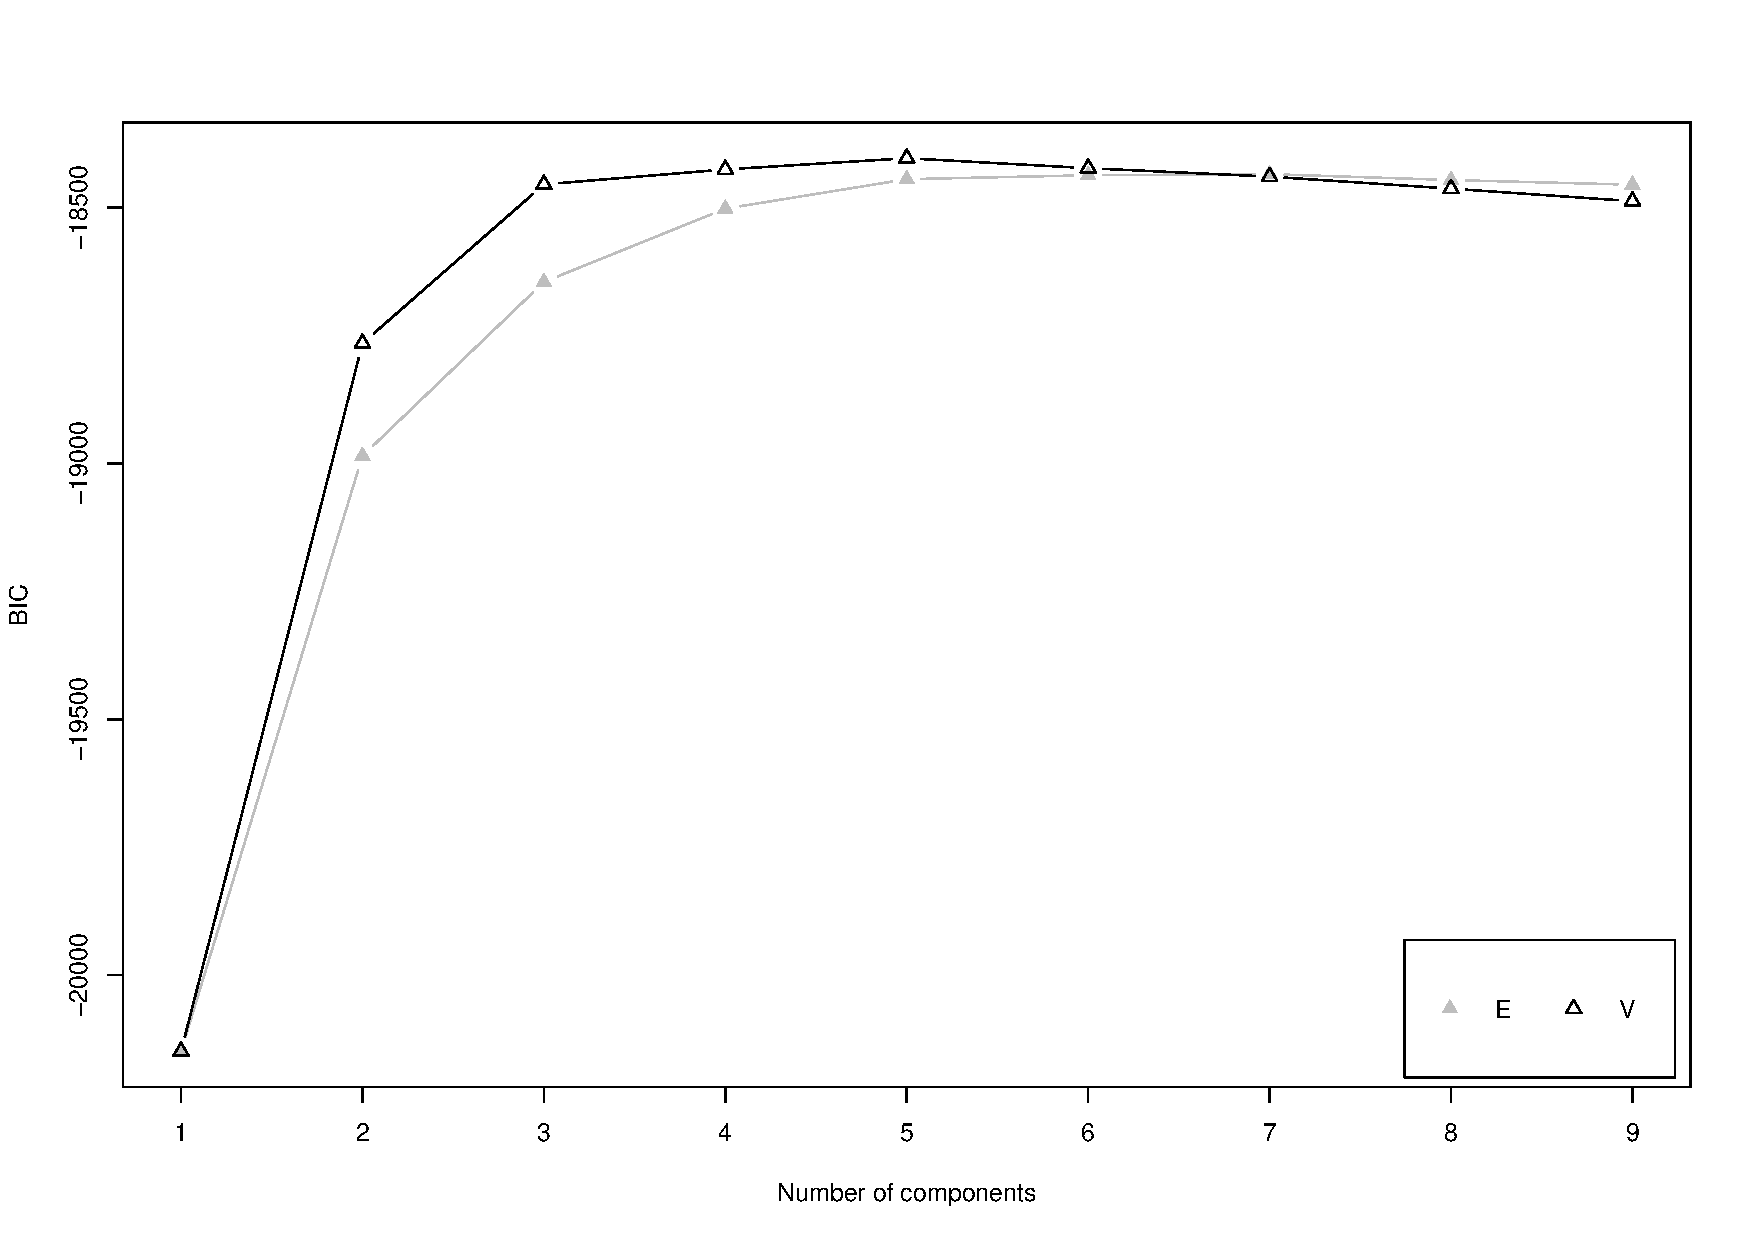
\includegraphics[width=\linewidth]{BIC}
\caption{BIC for several numbers of components}
\label{fig:BIC}
\end{marginfigure}

Fig.~\ref{fig:MixtureFit} shows the histogram, the individual components and the final model fit to the \verb|rms_hist75| data set.

\begin{marginfigure}
\centering
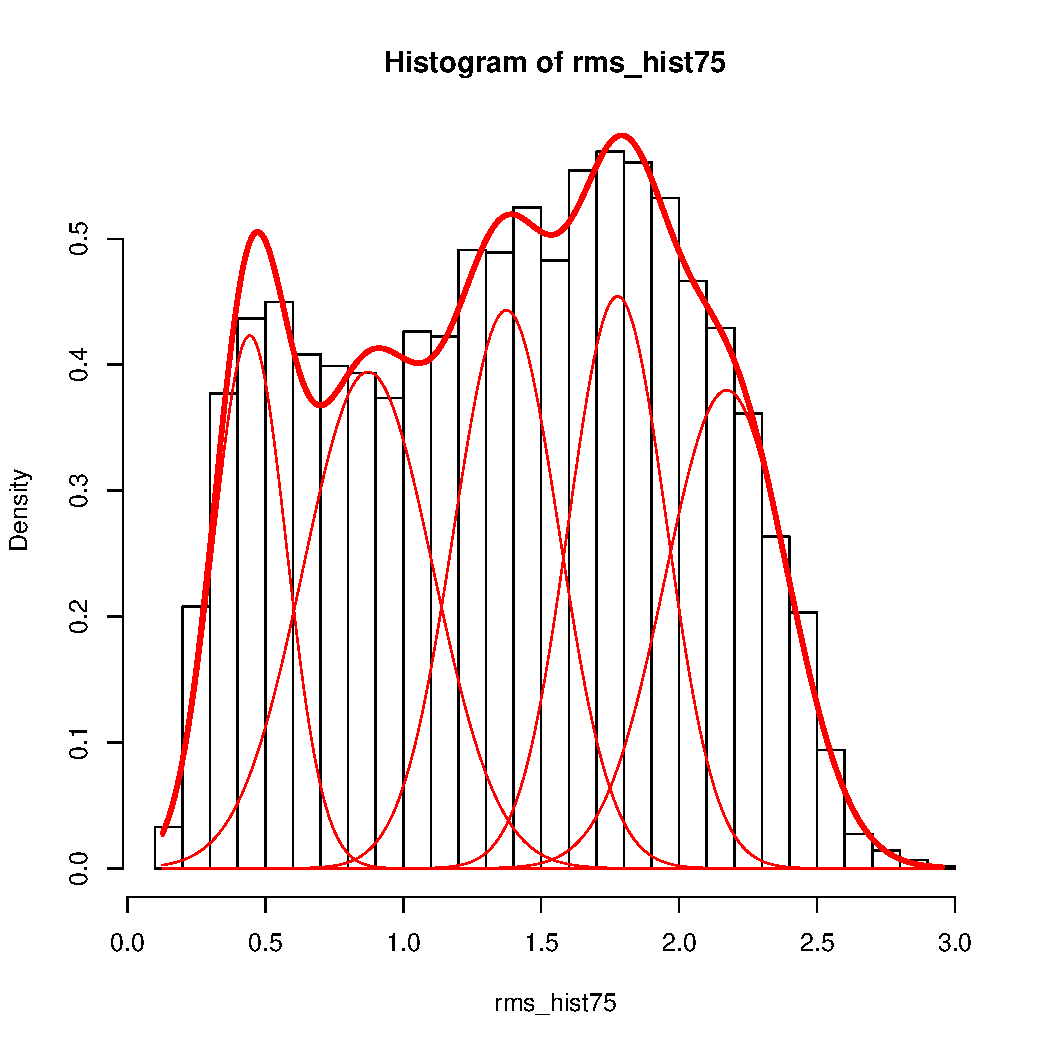
\includegraphics[width=\linewidth]{rms_hist75}
\caption{Histogram, individual components and resulting mixture model}
\label{fig:MixtureFit}
\end{marginfigure}


\subsection{The (SAR) Gamma distribution}

The likelihood function is 
\begin{align}
\mathcal L(L,\mu;\bm Z) =& \prod_{i=1}^{n}f_\Gamma(L,\mu; Z_i) = \prod_{i=1}^{n}\frac{L^L}{\mu^{L}\Gamma(L)} Z_i^{L-1} 
	\exp\big\{ -L Z_i / \mu
	\big\} \nonumber\\
	& = 
	\bigg(
	\frac{L^L}{\mu^{L}\Gamma(L)}
	\bigg)^n \prod_{i=1}^{n} \Big[Z_i^{L-1} \exp\big\{ -L Z_i / \mu
		\big\} \Big].
\end{align}
This is a very tough function to maximize.

A usual trick is taking the logarithm, as the likelihood function is positive.
One then obtains the ``complete log-likelihood function'':
\begin{equation}
\ell^*(L,\mu;\bm Z)=n\big[L(\log L - \log\mu) - \log\Gamma(L)
\big] + (L-1)\sum_{i=1}^n \log Z_i - \frac{L}{\mu} \sum_{i=1}^n Z_i.
\end{equation}
But there are terms that do not depend on either $L$ or $\mu$ and, therefore, are irrelevant for our maximization problem.
We are finally interested in the ``reduced log-likelihood function'':
\begin{equation}
\ell(L,\mu;\bm Z)=n\big[L(\log L - \log\mu) - \log\Gamma(L)
\big] + L\sum_{i=1}^n \log Z_i - \frac{L}{\mu} \sum_{i=1}^n Z_i.
\label{eq:RedLogLikGammaSAR}
\end{equation}

The maximum likelihood estimator of $(L,\mu)$ is then any point in $\mathbbm R_+^2$ satisfying
\begin{equation}
\widehat{(L,\mu)} = \arg\max_{(L,\mu)\in\mathbbm R_+^2} \ell(L,\mu;\bm Z).
\end{equation}

This problem can be solved in two ways: either deriving, equating to zero and solving, or by direct maximization.
Each case must be studied from a computational viewpoint to choose the most suitable option.

\section{The $\mathcal G^0$ distribution}

Recall that the $\mathcal G^0$ distribution was proposed as a means to model data from textured and extremely textured areas.
Assume that some textureless areas have been identified and that, with these data, it was possible to obtain a dependable estimate of $L$, say $\widehat L$.
As this equivalent number of looks should be valid for the whole image, we will consider it know when fitting data from textured areas.

Assume, then, that we have a sample $\bm Z = (Z_1,\dots,Z_n)$ of iid random variables that follow the $\mathcal G^0(\alpha,\gamma,\widehat L)$ distribution.
The unknown parameter $\theta=(\alpha,\gamma)$ lies in $\Theta=\mathbbm R_- \times \mathbbm R_+$.

The maximum likelihood estimator of $(\alpha,\gamma)$, is any point that maximizes the reduced log-likelihood:
\begin{equation}
\ell(\alpha,\gamma;\widehat L, \bm Z) = 
\frac{\Gamma(\widehat L-\alpha)}{\gamma^\alpha \Gamma(-\alpha)} +
\widehat L \sum_{n=1}^N \log\frac{Z_n}{\gamma+\widehat L Z_n} + 
\alpha \sum_{n=1}^N \log(\gamma + \widehat L Z_n),
\label{Eq:ReducedLogLikGI0}
\end{equation}
provided it lies in $\Theta$.
Maximizing~\eqref{Eq:ReducedLogLikGI0} might be a difficult task, in particular in textureless areas where $\alpha\to-\infty$ and the $\mathcal G^0$ distribution becomes very close to a Gamma law.
Small samples also pose difficult numerical problems, as $\ell$ becomes flat\cite{FreryCribariSouza:JASP:04}.

Most algorithms for maximizing~\eqref{Eq:ReducedLogLikGI0} require a starting point.
A good solution consists in using estimates obtained with the method of moments, i.e.\ by forming a system of two equations with suitable different values of $k$ in~\eqref{Eq:MomentGI0}.

\section{Analogy vs.\ Maximum Likelihood}

These methods should not be seen as competitors; they are complementary.

Analogy is usually more straightforward than Maximum Likelihood.
In particular, it does not require the expression of the density of the model (think, for instance, in the problem of estimating the parameter of the sum of $k$ random variables with $\mathcal U_{(0,\theta)}$ distribution).
Analogy leads to finding the roots of a system of (usually nonlinear) equations, and this is usually cumbersome in high-dimensional parametric spaces.

Estimators derived by Maximum likelihood have many asymptotic properties, and they are regarded to as the best ones for large samples when there is no contamination.
They can be obtained by either finding the roots of a system of (again, usually nonlinear) equations, which shares the problems of Analogy, or by optimization of the reduced log-likelihood function.
There are a number of excellent algorithms for the latter approach, numerical optimization\cite{maxLik}, EM and Simulated Annealing among them.

One frequently uses an analogy estimate as the starting point for optimization techniques that seek the maximum likelihood estimate.

\section{Improvement by bootstrap}

Bootstrap is a resampling technique.
We will see its simplest version.

Consider you have $\widehat{\theta}$, an estimator of $\theta$ based on the sample $\bm X=(X_1,\dots,X_n)$.

Its bias is $B(\widehat{\theta})=\operatorname{E}\widehat{\theta}-\theta$.

A better estimator would be, in terms of bias,
\begin{align}
\dot{\theta}	&=\widehat{\theta}-B(\theta)\\
				&=\widehat{\theta}- \operatorname{E}\widehat{\theta}+\theta\nonumber\\
				&=\widehat{\theta}+\theta-\operatorname{E}\widehat{\theta},
\end{align}
but we know neither $\theta$ nor $\operatorname{E}\widehat{\theta}$.

What do we do, as statisticians, when we do not know a quantity?
We estimate it!
So we propose the following estimator
\begin{align}
\widetilde{\theta}(\bm X) &= \widehat{\dot{\theta}} = \widehat{\theta} + \widehat{\theta} - \widehat{\operatorname{E}\widehat{\theta}} \nonumber\\
 &= 2\widehat{\theta} - \frac1R\sum_{r=1}^{R} \widehat{\theta}(\bm X^{(r)}),
\end{align}
where $\bm X^{(r)}$ is the result of resampling $\bm X$ with replacement.

In spite of seeming na\"ive and ad hoc, it has solid theoretical foundations and, more often than not, the bootstrap estimator is excellent, specially for relatively small samples\cite{CribariFrerySilva:CSDA,%
VasconcellosFrerySilva:CompStat,%
SilvaCribariFrery:ImprovedLikelihood:Environmetrics}.

\section{Comparison of estimators}

Assume you have two estimators, say $\widehat{\theta}$ and $\widetilde{\theta}$.
Denote any of them by $\dot\theta$.
They can be compared according to:
\begin{itemize}
\item their bias $B(\dot{\theta},\theta)=\operatorname{E}\dot\theta-\theta$,
\item their variance $\operatorname{Var}\dot{\theta}$,
\item their mean quadratic error $\operatorname{MQE}(\dot{\theta}) = \operatorname{E}(\dot{\theta-\theta})^2$,
\item are they fast and easy to compute?,
\item how fast they converge to the true value?,
\item do they converge, and how fast, to a Gaussian distribution?, and
\item are they robust before different types of contamination?
\end{itemize}
See details in \citet{busto92}.
Variance and bias should be as small as possible.
They must always be checked, either analytically (the ideal scenario), or by a well-designed Monte Carlo study.

\section*{Exercises}

All exercises must be solved as a report including a theoretical discussion, implementation details, careful (and visually appealing) plots, and conclusions.

\begin{exer}\label{Ex:Uiid}
Consider $\bm U=(U_1,\dots,U_n)$, a sample of iid $\mathcal U_{(0,\theta)}$ random variables with $\theta>0$ unknown.
Obtain at least three estimators for $\theta$ by the method of moments.
Compare them, in terms of bias and mean quadratic error, with respect to the maximum likelihood estimator.
Use a variety of sample sizes and true values of $\theta$.
\end{exer}

\begin{exer}
Improve all estimators obtained in Exercise~\ref{Ex:Uiid} by bootstrap.
Experiment with different bootstrap replications.
Consider also execution times.
\end{exer}

\begin{exer}
Consider the model given in~\eqref{eq:DensMixtureGaussian} such that $p=2$, $\mu_1=-1$, $\mu_2=1$, $\sigma_1^2=\sigma_2=1$, and $p_1=1/2$.
Write a routine for sampling from this model.
Now work with three situations of unknown means and variances:
(i)~one component, (ii)~two components, and (iii)~three components.
Assess the BIC of each situation by means of a Monte Carlo experiment, varying the sample size; you may use \num{1000} replications for each situation.
\end{exer}

\begin{exer}\label{Ex:Gammaiid}
Compare the maximum likelihood and a moment estimator for the model given in~\eqref{eq:SARGammaDensity} by means of a Monte Carlo experiment, using the bias and the mean quadratic error as measures of quality.
Consider a variety of true parameters and sample sizes.
\end{exer}

\begin{exer}
Extend Exercise~\ref{Ex:Gammaiid} by including bootstrap-improved estimators.
Make a global comparison.
\end{exer}

\begin{exer}\label{Ex:KIiid}
Find at least two estimators for the model given by~\eqref{Eq:DensKI}.
Compare them for a variety of parameters.
\end{exer}

\begin{exer}
Extend Exercise~\ref{Ex:KIiid} by including bootstrap-improved estimators.
Make a global comparison.
\end{exer}
